\chapter{Introduction}\label{ch:intro}

\section{Overview}\label{sec:intro-overview}
Computer vision gives machines the ability to interpret images and video. One of its central tasks is object detection: for each image, a detector returns the objects of interest as bounding boxes, each with a class label and a confidence score that expresses how sure the detector is about the box. Detection has moved from hand-crafted features to convolutional neural networks (CNNs) and, more recently, to transformer models \cite{li2025motreview,ren2017fasterrcnn,redmon2016yolo,carion2020detr}, and real-time detectors are now available for a wide range of hardware \cite{ismail2026realtime}.

Multi-object tracking (MOT) extends detection over time. It finds every object of interest in a video and gives each one an identity number (ID) that stays the same while the object is visible. MOT is a basic function of surveillance, traffic monitoring, driver assistance, and drone systems \cite{zhu2022visdrone,wu2022uavsurvey,geiger2012kitti}, where the results are usually needed with little delay. Unmanned aerial vehicles (UAVs) are a particularly demanding setting. They are used for traffic monitoring, surveillance, and search, and many of these tasks need every object to be detected in every frame and to keep the same identity over time \cite{wu2022uavsurvey,zhu2022visdrone}. Aerial video makes this difficult: objects are small, their number changes quickly, the camera moves, and illumination and blur change within one video \cite{zhu2022visdrone,du2018uavdt,cheng2023smallobject}.

Most MOT systems follow the tracking-by-detection design \cite{adzemovic2026survey,bewley2016sort,zhang2022bytetrack,ismail2026realtime}. In each frame, a detector returns candidate boxes with their scores, and an online tracker links these boxes into tracks, one per object. The two parts are developed separately and combined freely: any detector can feed any tracker. Their interaction is governed by a small number of settings that decide which boxes are used (Fig.~\ref{fig:intro-pipeline}). The detector removes boxes whose score is below its confidence threshold, removes overlapping boxes with non-maximum suppression (NMS), and resizes every frame to one input resolution; these three values form the \emph{detector operating point}. The tracker, in turn, uses a box only if its score passes its own thresholds: one score to match a box to an existing track, one score to start a new track, and, in two-stage trackers such as ByteTrack, a lower score for a second matching step \cite{zhang2022bytetrack}. In almost every system these settings are fixed once, for one detector and one type of scene, and they stay the same for the whole video.

\begin{figure}[tbp]
\centering
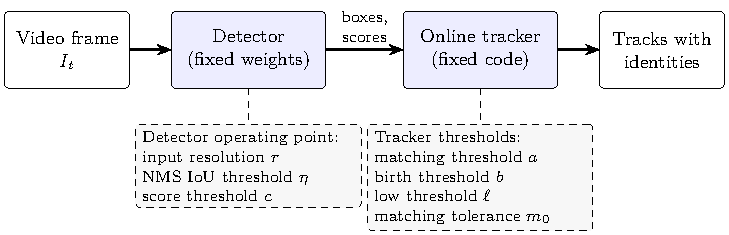
\includegraphics[width=0.95\textwidth]{figures/tbd_pipeline.pdf}
\caption{Tracking-by-detection pipeline and its operating points. The detector settings decide which boxes reach the tracker, and the tracker thresholds decide which of these boxes may match or start a track. In common practice all of these values are fixed for the whole video.}
\label{fig:intro-pipeline}
\end{figure}

The reliability of a tracking system therefore depends not only on the quality of its detector and tracker, but also on whether these fixed settings fit the scene and the detector that are actually present. Two situations break this fit in practice. Within one aerial video, the scene changes from sparse to crowded, from clear to blurred, and from large to tiny objects. Across the life of a system, the detector is replaced, retrained, or compressed, while the tracker keeps the thresholds that its authors tuned for another detector.

This thesis addresses real-time target detection and tracking and follows one research direction through three studies. A survey of real-time object detection and tracking, published by the author \cite{ismail2026realtime}, reviewed the detectors, trackers, datasets, and metrics of the field, showed that tracking by detection remains the dominant paradigm, and identified the accuracy--speed trade-off, the hardware, and the deployment environment as the main constraints of real-time operation. Building on this review, the thesis treats the settings that connect the detector and the tracker as control variables of the tracking system rather than as fixed parameters, and it proposes two training-free controllers that adapt them online with the detector and the tracker left unchanged. The first, Adaptive Control for Multi-Object Tracking (AC-MOT), adapts the detector operating point to the changing aerial scene (Chapter~\ref{ch:acmot}). The second, a self-calibrating control layer (SCL), adapts the candidates, scores, and thresholds that a tracker receives to the score scale of the detector in use (Chapter~\ref{ch:scl}).

\section{Motivation and Challenges}\label{sec:intro-motivation}
The motivation of this thesis comes from the three studies on which it is built. The survey identified the general difficulties of real-time detection and tracking \cite{ismail2026realtime}; the AC-MOT and SCL studies then measured, on public benchmarks, how strongly two of these difficulties affect a working tracking pipeline. In the following, statements supported by the literature are separated from effects that are demonstrated by the experiments of this thesis.

\emph{Variable scene complexity.} Aerial video changes within a single sequence: object density, object size, illumination, and blur vary with the flight path, the altitude, and the viewing angle \cite{zhu2022visdrone,du2018uavdt}. A setting that works in a sparse, clear scene can keep too much clutter in a dense scene, and a setting that works in a dense scene can lose small or weak objects in another part of the same video. A fixed operating point is therefore a compromise over all the scenes of a video.

\emph{Small and crowded objects.} Small objects occupy few pixels and usually receive low detector confidence \cite{cheng2023smallobject}. In crowded scenes, individual objects are hard to separate, and occlusion causes missed detections and identity switches \cite{li2025motreview,ismail2026realtime}. A larger input resolution helps small objects, but it costs the same detector time on easy and hard frames.

\emph{Motion, occlusion, and image degradation.} The motion of a UAV camera moves the boxes of all objects between frames, which the motion model of a tracker must absorb \cite{liu2022uavmot}. Severe occlusion, illumination changes, blur, and weather reduce the recall of the detector and change the distribution of its confidence scores \cite{chae2024radar,ismail2026realtime}.

\emph{Sensitivity to the detector operating point.} The choice of the confidence threshold, the NMS threshold, and the input resolution moves false detections, missed objects, identity switches, and runtime together. This effect is demonstrated in Chapter~\ref{ch:acmot}: with the same frozen detector and the same trackers on the same aerial sequences, changing only the operating point raised the multiple object tracking accuracy (MOTA) by 17.995 points with ByteTrack and by 6.318 points with OATrack.

\emph{Tracker dependence on detection scores.} Trackers read detector scores through fixed thresholds that their authors tuned for one detector, usually YOLOX \cite{ge2021yolox} on the MOT17 benchmark. Detector scores, however, are not calibrated across models and conditions \cite{guo2017calibration,kuppers2020detcalib}, so a new detector usually gives scores on a different scale, and nothing in the system notices. The effect is demonstrated in Chapter~\ref{ch:scl}: ByteTrack in its official setting starts a track only from a box with a score of at least 0.7; when the scores of a published detector are halved, a car that was scored 0.9 now gets 0.45, ByteTrack never starts a track, and its higher order tracking accuracy (HOTA) \cite{luiten2021hota} falls from 67.70 to 0.

\emph{Variation between detectors, trackers, and datasets.} The best setting depends on the combination of components. In this thesis, a tracker that uses low-score boxes in a second association step reacted differently to the same detector control than a tracker that weights detections by quality (Chapter~\ref{ch:acmot}), and single-stage and two-stage trackers needed different help when the detector changed (Chapter~\ref{ch:scl}). With a replacement detector, the real-time detection transformer RT-DETR-L, ByteTrack in its published setting reached a MOTA of only 3.29 on held-out aerial data (Chapter~\ref{ch:scl}).

\emph{Limits of fixed configurations and of existing adaptation.} Retuning every detector--tracker pair for every deployment needs labelled data, which a deployed system does not have. Methods that adapt the detector at run time usually learn their policy with an extra model for one detector \cite{han2022dynamic,chin2019adascale,xu2020approxdet}; methods that adapt tracker thresholds are each built into one tracker \cite{ma2023adaptivebytetrack,shim2024adaptrack,act2026adaptive}; and score calibration fits a mapping on labelled data \cite{kuppers2020detcalib}. None of these generalizes directly to a new combination of detector, tracker, and scene without training or labels.

These observations lead to the challenges that an online controller of the operating point must meet:
\begin{itemize}
\item \emph{No labels at run time.} A deployed system has no ground truth, so the adaptation must be decided from the video and from the system's own outputs.
\item \emph{Causality and low cost.} Only the current and earlier frames may be used, and the extra computation must be small next to the detector, so that the system stays usable in real time.
\item \emph{Unchanged components.} Retraining the detector or rewriting the tracker for every new combination is costly and loses the modularity of tracking by detection; the controller should work from the outside.
\item \emph{Stability.} Each change of the operating point changes the boxes that reach the tracker, so the settings should follow lasting changes of the scene rather than single frames.
\item \emph{No harm when nothing is wrong.} A tracker that already fits its detector should keep its accuracy; an adaptation that always intervenes can lower it (Section~\ref{sec:scl-prior}).
\end{itemize}

\section{Problem Statement}\label{sec:intro-problem}
Let a video be a sequence of frames $I_1, I_2, \dots$, processed online by a frozen detector and a frozen tracker. The weights of the detector, and the code and association algorithm of the tracker, are not changed. At frame $t$, the detector runs with an operating point $\theta_t=(c_t,\eta_t,r_t)$, its confidence threshold, NMS threshold, and input resolution, and returns candidates $D_t$, each with a box, a score, and a class. The tracker reads these candidates through its published thresholds and returns the tracks of frame $t$. A controller may set only values that the pipeline already exposes, and it may base its decision only on the current frame, on earlier frames, and on the outputs that the detector and the tracker have already produced. No ground truth, no future frame, and no training is allowed. The goal is to improve tracking accuracy, measured by HOTA, MOTA, the identity F1 score (IDF1), and the number of identity switches (IDS), relative to the same pipeline with fixed settings, while adding little computation.

Existing work does not solve this problem as stated. Adaptive inference methods change the detector configuration, but they learn a policy for one model and optimize detection rather than tracking; adaptive-threshold methods adapt one tracker to the current frame; and calibration methods need labels (Section~\ref{sec:rw-gap}). The thesis therefore addresses three research questions (RQ1--RQ3):
\begin{enumerate}
\item[\textbf{RQ1}] Can the detector operating point be adapted online from inexpensive scene cues and the past output of the tracker, without training, so that tracking in aerial video improves over a fixed operating point with the detector and the trackers unchanged? (Chapter~\ref{ch:acmot})
\item[\textbf{RQ2}] Can a label-free and causal layer decide from recent detector scores whether the score scale of a detector fits the published thresholds of a tracker, leave a well-matched pair as it is, and restore a mismatched pair through the tracker's own published settings? (Chapter~\ref{ch:scl})
\item[\textbf{RQ3}] Do the effects of the frozen controllers hold on data, trackers, and detectors that were not used to design them, at a cost compatible with real-time operation? (Chapters~\ref{ch:acmot} and~\ref{ch:scl})
\end{enumerate}

The two research questions RQ1 and RQ2 describe two related but distinct problems. The first is narrower: it concerns one place in the pipeline, the detector call, in one setting, UAV video with one detector, and it assumes that the scores of the detector keep the scale for which the tracker thresholds were set. Its controller, AC-MOT, is formulated in Chapter~\ref{ch:acmot} as a control rule $\theta_t=\pi(I_t,\mathcal{B}_{1:t-1})$ that selects the operating point from the current image and the boxes tracked in earlier frames. The second problem is more general: it removes that assumption and asks how one fixed set of rules can make the scores of any detector usable by different published trackers. Its controller, SCL, is formulated in Chapter~\ref{ch:scl} as a layer that maps the score logits of earlier frames, the current candidates, the previous tracks, and the camera motion to the candidates, scores, thresholds, and matching tolerance that the tracker receives. The two controllers act at different points of the pipeline and are not two versions of one algorithm: AC-MOT does not adapt the tracker thresholds, and SCL does not choose the detector operating point. Each was developed and evaluated on its own, and neither replaces the other.

\section{Solution Approach}\label{sec:intro-solution}
The thesis answers these questions with two rule-based controllers that share the same principles: no learned weights, no labels at run time, use of past information only, an unchanged detector and tracker, values fixed before the final evaluation, and paired bootstrap statistics for every comparison. Figure~\ref{fig:intro-outline} shows where they act, and Table~\ref{tab:intro-controllers} compares their scope.

\begin{figure}[tbp]
\centering
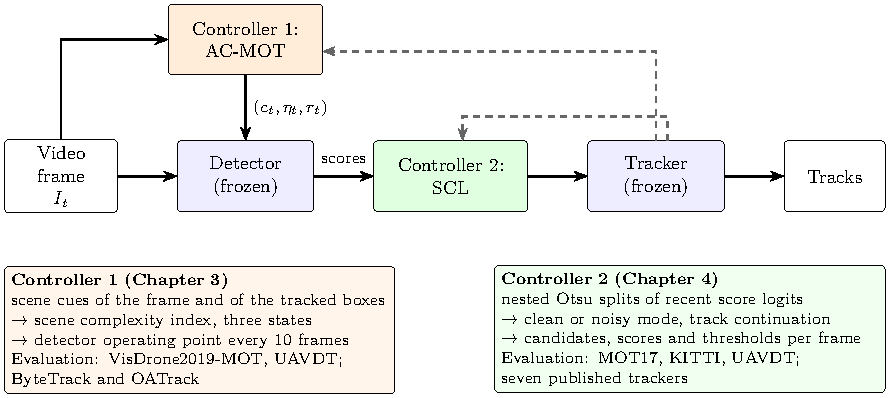
\includegraphics[width=0.98\textwidth]{figures/outline.pdf}
\caption{Outline of the proposed approach. Controller~1 (AC-MOT) sets the detector operating point from scene cues; Controller~2 (SCL) adapts the candidates, scores, and thresholds that the tracker receives from the detector's score distribution. Dashed arrows: tracked boxes of the previous frame.}
\label{fig:intro-outline}
\end{figure}

\emph{A. AC-MOT: online control of the detector operating point.} AC-MOT runs next to the detector. On the first frame and then on every tenth frame, it measures inexpensive cues of the current image and of the boxes that the tracker reported in the previous frame, averages the recent crowd level into a scene complexity index (SCI), and selects one of three detector operating points through a three-state controller with recovery, hysteresis, and dwell rules. Its output is the confidence threshold, the NMS threshold, and the input resolution of the detector until the next analysis step. Its thresholds and actions were selected by cross-validation on separate calibration sequences and then frozen. It assumes a detector that can be run at the three selected operating points and a tracker whose boxes can be read after each frame; it was evaluated on UAV video with one detector and two trackers.

\emph{B. SCL: a self-calibrating layer between the detector and the tracker.} SCL runs once per frame between the detector and the tracker. It splits the score logits of the last ten frames twice with Otsu's method \cite{goh2018otsu} into background, uncertain, and confident groups, and decides from the share of confident candidates whether the score distribution is clean or noisy. On clean scores it keeps the tracker's scores and thresholds and lowers a threshold only if it would reject the confident group; on noisy scores it chooses the candidates, gives them new scores, and sets the thresholds. A track-guided recovery lets a weak box that clearly continues a track reach single-stage trackers, which have no low-score step of their own, and the matching tolerance follows strong camera motion. The layer serves different published trackers through four of their published settings, called the host contract. Its outputs are the candidates, their scores, the thresholds, and the matching tolerance of the tracker for each frame. It assumes that the order of the scores carries information about the objects, and that a tracker publishes the four values of its contract; it was evaluated with seven trackers, four detection sources, and three datasets.

\begin{table}[tbp]
\centering
\caption{The two controllers of this thesis: where they act, what they read and set, and how their values were chosen.}
\label{tab:intro-controllers}
\begin{tabular}{>{\raggedright\arraybackslash}p{2.9cm}>{\raggedright\arraybackslash}p{5.5cm}>{\raggedright\arraybackslash}p{5.5cm}}
\toprule
Aspect & AC-MOT (Chapter~\ref{ch:acmot}) & SCL (Chapter~\ref{ch:scl})\\
\midrule
Acts on & detector operating point: confidence threshold, NMS threshold, input resolution & tracker input: candidates, scores, thresholds, matching tolerance\\
Reads & image cues of the current frame and tracked boxes of the previous frame & score logits of the last 10 frames, tracks of the previous frame, camera motion, host contract\\
Update & every 10 frames & every frame\\
Decision & three states from the scene complexity index, with recovery, hysteresis, and dwell & clean or noisy mode from nested Otsu splits and a whole-stream median\\
Values chosen by & cross-validation on calibration sequences & standard values and design choices, no search\\
Unchanged parts & detector weights, tracker & detector, tracker code and association\\
Evaluated on & VisDrone2019-MOT and UAVDT, ByteTrack and OATrack & MOT17, KITTI, and UAVDT, seven published trackers\\
\bottomrule
\end{tabular}
\end{table}

The two controllers form one research narrative. The survey established that tracking by detection is the dominant paradigm and that detection accuracy and association reliability depend on each other \cite{ismail2026realtime}. AC-MOT showed that the detector operating point is a first-order variable of aerial MOT that can be controlled online without training. SCL then addressed the assumption that AC-MOT still makes, a fixed relation between the detector's scores and the tracker's thresholds, and showed that this compatibility can be checked and restored online for different trackers.

The contributions of this research are as follows:
\begin{itemize}
\item A structured, deployment-oriented survey of real-time object detection and tracking, published at IEEE ICMISI 2026 \cite{ismail2026realtime}, which forms the basis of the technical background in Chapter~\ref{ch:background}.
\item AC-MOT, a training-free and causal controller that treats the detector operating point as part of the MOT system and adapts it online, with the detector and the tracker unchanged, together with an optimization-guided development path whose final values are selected by cross-validation on calibration sequences \cite{ismail2026acmot}.
\item An evaluation of AC-MOT on VisDrone2019-MOT with two trackers, ByteTrack and OATrack, using eight MOT metrics and paired bootstrap intervals, and a transfer to UAVDT without retuning.
\item SCL, a training-free and causal layer whose novelty is selective, host-aware adaptation: it keeps the tracker's scores and thresholds when the scores are clean, takes control only when they are noisy, and expresses every action through a host contract that lets one fixed configuration serve single-stage and two-stage trackers without changing them \cite{ismail2026scl}.
\item An evaluation of one frozen SCL configuration on seven published trackers, four detection sources, and three datasets, including score shifts, predeclared external trackers, a held-out aerial test split, comparisons with simple adaptive thresholds and the published ACT method, an ablation, and a sensitivity analysis.
\item Runtime measurements showing that both controllers add only a few milliseconds per frame.
\end{itemize}
The detectors, the trackers, Otsu's method, and the phase correlation used by SCL are existing methods and are used unchanged; the contributions lie in the control rules, in the way they connect existing components, and in their evaluation. The survey has been published; the AC-MOT and SCL manuscripts have been submitted and are under review (see Publications).

\section{Thesis Organization}\label{sec:intro-organization}
The rest of this thesis is organized as follows.

\textbf{Chapter 2: Background and Related Work}

This chapter provides the technical background needed for the two controllers: object detection, deep learning-based detectors, MOT and its paradigms, data association and track management, detector confidence and thresholding, aerial tracking and the datasets of the thesis, and the evaluation metrics and protocols. It then reviews the related work on tracking-by-detection systems, adaptive inference, adaptive thresholds, and score calibration, compares the closest methods, and states the research gap.

\textbf{Chapter 3: AC-MOT: Adaptive Detector Operating-Point Control}

This chapter formulates the control of the detector operating point, presents the scene cues, the scene complexity index, the three-state controller, and the action map of AC-MOT, explains how its values were selected through optimization experiments on calibration data, and evaluates the frozen controller on VisDrone2019-MOT and, without retuning, on UAVDT.

\textbf{Chapter 4: SCL: Training-Free Self-Calibrating Control Layer}

This chapter formulates the compatibility between a detector's score scale and a tracker's thresholds, presents the five steps and the host contract of SCL and its development and freeze, and evaluates the frozen layer on seven trackers, four detection sources, and three datasets, with adaptive-threshold baselines, the ACT method, an ablation, a sensitivity analysis, and runtime measurements.

\textbf{Chapter 5: Conclusions and Future Work}

This chapter draws the conclusions of the thesis as a whole, summarizes the findings and the scope of the two controllers, and outlines directions for future work.
